\documentclass[]{elsarticle} %review=doublespace preprint=single 5p=2 column
%%% Begin My package additions %%%%%%%%%%%%%%%%%%%
\usepackage[hyphens]{url}

  \journal{Transport Findings} % Sets Journal name


\usepackage{lineno} % add
\providecommand{\tightlist}{%
  \setlength{\itemsep}{0pt}\setlength{\parskip}{0pt}}

\usepackage{graphicx}
\usepackage{booktabs} % book-quality tables
%%%%%%%%%%%%%%%% end my additions to header

\usepackage[T1]{fontenc}
\usepackage{lmodern}
\usepackage{amssymb,amsmath}
\usepackage{ifxetex,ifluatex}
\usepackage{fixltx2e} % provides \textsubscript
% use upquote if available, for straight quotes in verbatim environments
\IfFileExists{upquote.sty}{\usepackage{upquote}}{}
\ifnum 0\ifxetex 1\fi\ifluatex 1\fi=0 % if pdftex
  \usepackage[utf8]{inputenc}
\else % if luatex or xelatex
  \usepackage{fontspec}
  \ifxetex
    \usepackage{xltxtra,xunicode}
  \fi
  \defaultfontfeatures{Mapping=tex-text,Scale=MatchLowercase}
  \newcommand{\euro}{€}
\fi
% use microtype if available
\IfFileExists{microtype.sty}{\usepackage{microtype}}{}
\bibliographystyle{elsarticle-harv}
\ifxetex
  \usepackage[setpagesize=false, % page size defined by xetex
              unicode=false, % unicode breaks when used with xetex
              xetex]{hyperref}
\else
  \usepackage[unicode=true]{hyperref}
\fi
\hypersetup{breaklinks=true,
            bookmarks=true,
            pdfauthor={},
            pdftitle={An examination of the accessibility implications of a pilot COVID-19 vaccination program in Hamilton, Ontario},
            colorlinks=false,
            urlcolor=blue,
            linkcolor=magenta,
            pdfborder={0 0 0}}
\urlstyle{same}  % don't use monospace font for urls

\setcounter{secnumdepth}{0}
% Pandoc toggle for numbering sections (defaults to be off)
\setcounter{secnumdepth}{0}

% Pandoc citation processing

% Pandoc header
\usepackage{float} \usepackage{xcolor} \floatplacement{figure}{H}
\usepackage{booktabs}
\usepackage{longtable}
\usepackage{array}
\usepackage{multirow}
\usepackage{wrapfig}
\usepackage{float}
\usepackage{colortbl}
\usepackage{pdflscape}
\usepackage{tabu}
\usepackage{threeparttable}
\usepackage{threeparttablex}
\usepackage[normalem]{ulem}
\usepackage{makecell}
\usepackage{xcolor}



\begin{document}
\begin{frontmatter}

  \title{An examination of the accessibility implications of a pilot COVID-19
vaccination program in Hamilton, Ontario}
    \author[McMaster University]{Antonio Paez\corref{1}}
   \ead{paezha@mcmaster.ca} 
    \author[University of Toronto Scarborough]{Christopher D. Higgins}
   \ead{cd.higgins@utoronto.ca} 
      \address[McMaster University]{School of Earth, Environment and Society, McMaster University, Hamilton,
ON, L8S 4K1, Canada}
    \address[University of Toronto Scarborough]{Department of Geography \& Planning, University of Toronto Scarborough,
1265 Military Trail, Toronto, ON M1C1A4}
      \cortext[1]{Corresponding Author}
  
  \begin{abstract}
  The province of Ontario in Canada announced the pilot for a new
  vaccination program, with designated pharmacies across the province now
  able to offer COVID-19 vaccines. The accessibility of this program
  raises questions about the cost of travel and the distribution of the
  cost among the population. In our examination of the City of Hamilton we
  find that selected sites do not serve well the rural and urban
  population of Hamilton, and that the associated cost of travel is
  expected to be disproportionally borne by lower income populations.
  Modest additions to the list of pilot sites in the city can
  substantially alleviate this inequity.
  \end{abstract}
  
 \end{frontmatter}

\hypertarget{research-questions-and-hypotheses}{%
\section{Research Questions and
Hypotheses}\label{research-questions-and-hypotheses}}

Along with the provision of health care facilities to treat severe cases
of COVID-19 (Pereira et al., 2021), another front in the fight against
the pandemic is the rolling out of vaccination programs. The Province of
Ontario, in Canada, announced on April 1st 2021 the expansion of a pilot
program to offer vaccines in pharmacies in the City of
Hamilton\footnote{\url{https://www.cbc.ca/news/canada/hamilton/astrazeneca-vaccine-hamilton-1.5972704}}.
This program is in addition to dedicated vaccination centers for people
aged 70+. Twenty pharmacies in Hamilton were added to an earlier list of
325 locations in other cities across the province, and the program was
extended to people aged 55 years old and over.

Critics were quick to point out that the list of pharmacies approved for
Hamilton were mostly located in lower density parts of the city that are
not well serviced by transit and are difficult to reach by
foot\footnote{See inter alia: \url{https://twitter.com/RyanMcGreal/status/1378027149790224386?s=20} and \url{https://twitter.com/NrinderWard3/status/1378679195514060801?s=20}.}.
Indeed, as seen in Figure \ref{fig:pharmacies-and-regions}, a vast
majority of the pharmacies are in suburban Hamilton. The issue is
somewhat less clear cut when we consider that Hamilton's suburbs tend to
be older (see Figure \ref{fig:population-map}). The population aged 55
to 69 in Hamilton is approximately 59,095 suburban, 35,704 urban, and
only 35,704 rural. Given the target demographic for the program, it is
possible that suburban sites could be convenient for mature and older
adults. Nevertheless, the selection of sites by the province raises some
important
questions\footnote{The decision-making process to select these sites appears to have been opaque, and the normally inert Major of the city was caught flat footed by the announcement; see:\url{https://twitter.com/FredEisenberger/status/1378350123114242053?s=20}}.
As Yu et al. (2021) note, good geographical coverage is a key element
for a successful vaccination campaign; at the same time, siting
vaccinations sites in car-oriented locations may introduce inequities in
access.

In this research, we investigate the accessibility implications of the
sites selected for the pilot vaccination program. Concretely, we ask:

\begin{itemize}
\tightlist
\item
  What is the estimated cost of travel to reach the vaccination sites,
  assuming that every person requires a vaccine?
\item
  What is the distribution of this cost across the population of the
  city?
\item
  How does the cost and its distribution change with the addition of
  candidate sites in urban Hamilton?
\end{itemize}

We concentrate on the 55 to 69 years old population segment because the
older 70+ group have access to other dedicated facilities besides those
in the provincial pilot.

\begin{figure}

{\centering 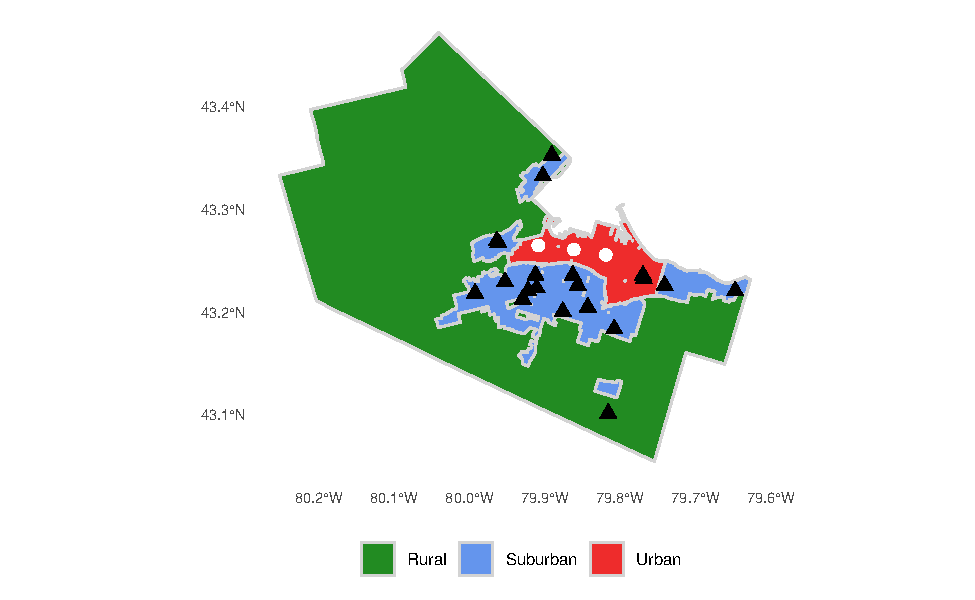
\includegraphics{Accessibility-Vaccination-Sites-Hamilton_files/figure-latex/pharmacies-map-1} 

}

\caption{\label{fig:pharmacies-and-regions}Location of pharmacies in pilot and regions with the City of Hamilton}\label{fig:pharmacies-map}
\end{figure}

\begin{figure}

{\centering 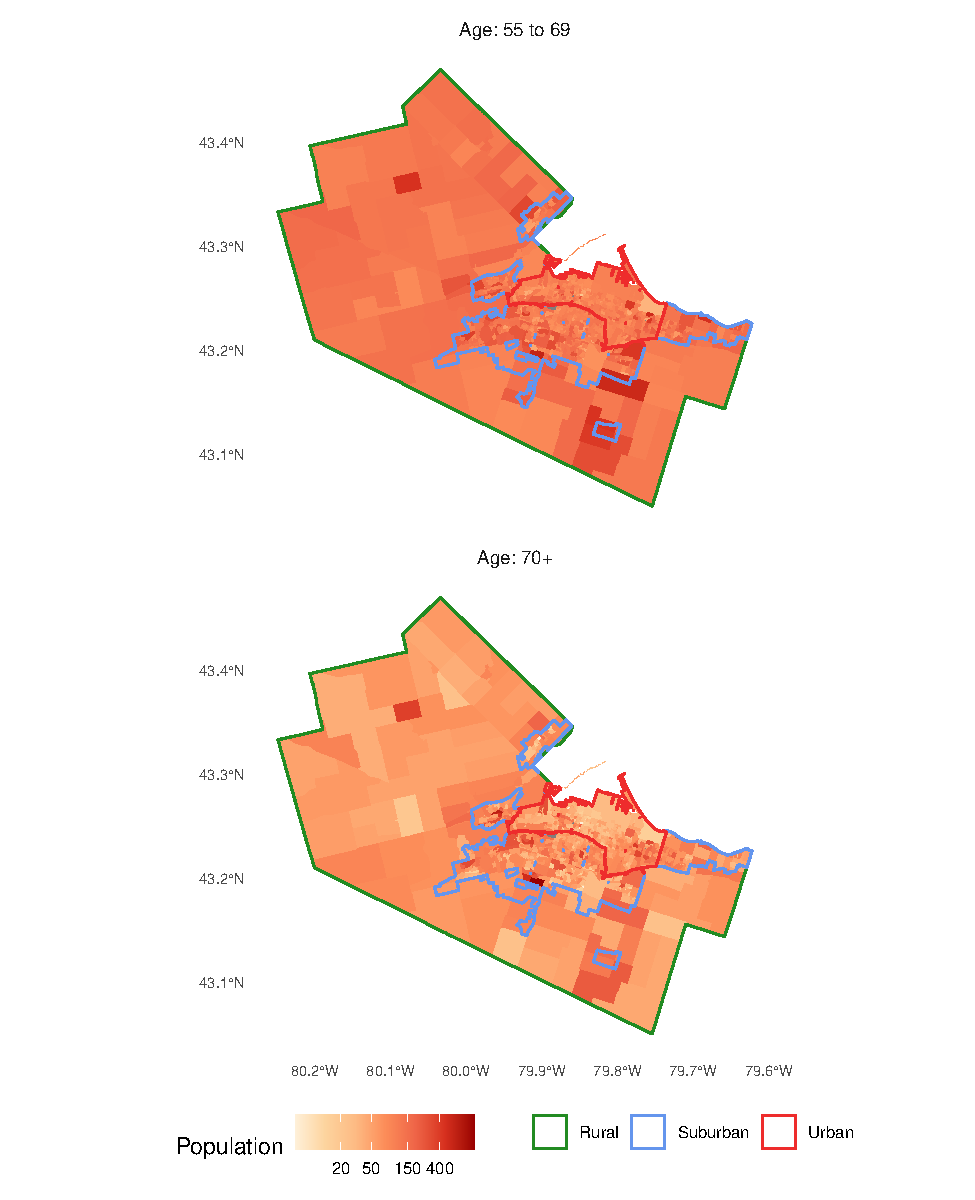
\includegraphics{Accessibility-Vaccination-Sites-Hamilton_files/figure-latex/population-map-1} 

}

\caption{\label{fig:population-map}Distribution of population age 55+ in the City of Hamilton}\label{fig:population-map}
\end{figure}

\hypertarget{methods-and-data}{%
\section{Methods and Data}\label{methods-and-data}}

This paper is a reproducible research document (see Brunsdon and Comber,
2020) conducted using open source tools for transportation analysis
(Lovelace, 2021). All code and data necessary to reproduce the tables
and figures are available in a public
repository\footnote{\url{https://github.com/paezha/Accessibility-Pharmacies-Hamilton-Vaccines}}.

\hypertarget{findings}{%
\section{Findings}\label{findings}}

Words.

\begin{figure}

{\centering 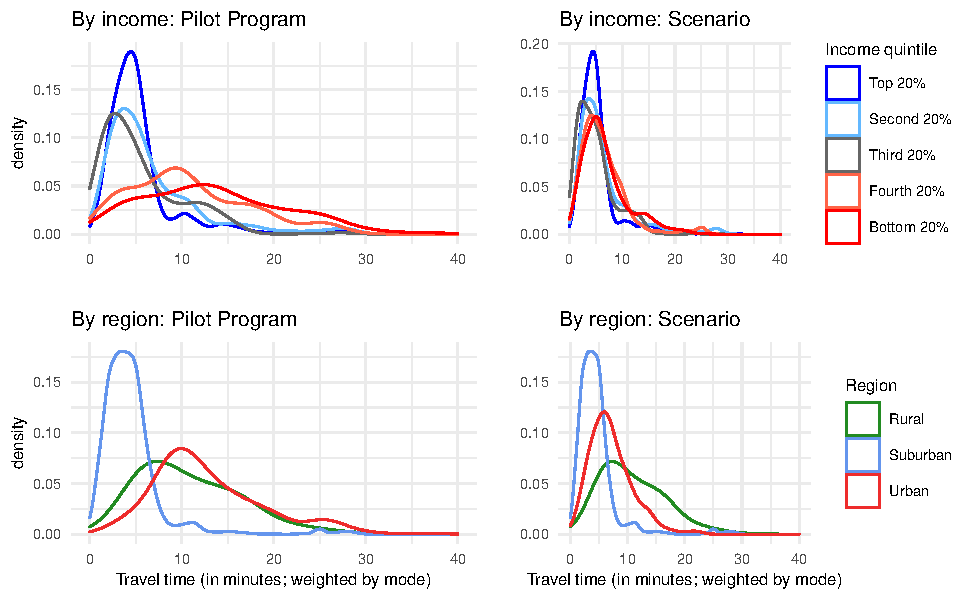
\includegraphics{Accessibility-Vaccination-Sites-Hamilton_files/figure-latex/figure-results-1} 

}

\caption{\label{fig:results}Distribution of travel time (weighted by mode) for different population groups}\label{fig:figure-results}
\end{figure}

\begin{table}

\caption{\label{tab:table-results}\label{tab:distribution-results}Distribution of person hours travelled (PHT) by median total household income and region: pilot locations only, and scenario with three urban locations added}
\centering
\resizebox{\linewidth}{!}{
\begin{tabular}[t]{lccccc}
\toprule
\multicolumn{2}{c}{ } & \multicolumn{2}{c}{Pilot Program} & \multicolumn{2}{c}{Scenario} \\
\cmidrule(l{3pt}r{3pt}){3-4} \cmidrule(l{3pt}r{3pt}){5-6}
Group & Population & Total PHT & Hours per person & Total PHT & Hours per person\\
\midrule
\addlinespace[0.3em]
\multicolumn{6}{l}{\textbf{Income Quintile}}\\
\hspace{1em}\cellcolor{gray!6}{Top 20\%} & \cellcolor{gray!6}{23297.315} & \cellcolor{gray!6}{2243.857} & \cellcolor{gray!6}{0.096} & \cellcolor{gray!6}{2146.558} & \cellcolor{gray!6}{0.092}\\
\hspace{1em}Second 20\% & 22356.413 & 2471.952 & 0.111 & 2351.858 & 0.105\\
\hspace{1em}\cellcolor{gray!6}{Third 20\%} & \cellcolor{gray!6}{19570.061} & \cellcolor{gray!6}{1749.497} & \cellcolor{gray!6}{0.089} & \cellcolor{gray!6}{1563.978} & \cellcolor{gray!6}{0.080}\\
\hspace{1em}Fourth 20\% & 17729.139 & 2928.959 & 0.165 & 1950.312 & 0.110\\
\hspace{1em}\cellcolor{gray!6}{Bottom 20\%} & \cellcolor{gray!6}{19629.952} & \cellcolor{gray!6}{4068.548} & \cellcolor{gray!6}{0.207} & \cellcolor{gray!6}{2388.422} & \cellcolor{gray!6}{0.122}\\
\addlinespace[0.3em]
\multicolumn{6}{l}{\textbf{Region}}\\
\hspace{1em}Rural & 8356.963 & 1730.268 & 0.207 & 1730.242 & 0.207\\
\hspace{1em}\cellcolor{gray!6}{Suburban} & \cellcolor{gray!6}{58711.629} & \cellcolor{gray!6}{4138.482} & \cellcolor{gray!6}{0.070} & \cellcolor{gray!6}{4138.392} & \cellcolor{gray!6}{0.070}\\
\hspace{1em}Urban & 35491.942 & 7588.590 & 0.214 & 4527.021 & 0.128\\
\bottomrule
\multicolumn{6}{l}{\rule{0pt}{1em}\textit{Note: }}\\
\multicolumn{6}{l}{\rule{0pt}{1em}The population totals differ due to small differences in the classification of the regions}\\
\end{tabular}}
\end{table}

\hypertarget{references}{%
\section*{References}\label{references}}
\addcontentsline{toc}{section}{References}

\hypertarget{refs}{}
\leavevmode\hypertarget{ref-Brunsdon2020opening}{}%
Brunsdon, C., Comber, A., 2020. Opening practice: Supporting
reproducibility and critical spatial data science. Journal of
Geographical Systems 1--20.

\leavevmode\hypertarget{ref-Lovelace2021open}{}%
Lovelace, R., 2021. Open source tools for geographic analysis in
transport planning. Journal of Geographical Systems.
doi:\href{https://doi.org/10.1007/s10109-020-00342-2}{10.1007/s10109-020-00342-2}

\leavevmode\hypertarget{ref-Pereira2021geographic}{}%
Pereira, R.H.M., Braga, C.K.V., Servo, L.M., Serra, B., Amaral, P.,
Gouveia, N., Paez, A., 2021. Geographic access to covid-19 healthcare in
brazil using a balanced float catchment area approach. Social Science \&
Medicine 273, 113773.
doi:\href{https://doi.org/https://doi.org/10.1016/j.socscimed.2021.113773}{https://doi.org/10.1016/j.socscimed.2021.113773}

\leavevmode\hypertarget{ref-Yu2021sustained}{}%
Yu, J.H., Jeong, H.J., Kim, S.J., Lee, J.Y., Choe, Y.J., Choi, E.H.,
Cho, E.H., 2021. Sustained vaccination coverage during the coronavirus
disease 2019 epidemic in the republic of korea. Vaccines 9, 8.
doi:\href{https://doi.org/10.3390/vaccines9010002}{10.3390/vaccines9010002}


\end{document}


